\chapter{Design}

\section{Introduction} % (fold)
\label{sec:introduction}

Today the web has become the central point of all applications. With presence of Internet, users can use many applications without needing to install the program on their machine. Technologies such as JavaScript, HTML, CSS are evolving rapidly and has been created an opportunity for the users of world wide web to have a more pleasant experience. Therefore fast and robust application plays an important role in attracting users and convincing them to migrate from installing the programs on their machine and instead use their browsers. In order to build robust web applications,  one must implement new state of the art software engineering designs.

\subsection{Purpose} % (fold)
\label{sub:purpose}

This chapter describes architecture design of `Virtual Assistance' application. It is intended to describe the design of the system fully enough to allow future contributors of the project to clearly understand of how the software is expected to be build. Design chapter will provide overview and description of the system and relations between the components and user interaction. 

\subsection{Scope} % (fold)
\label{sub:scope}
The scope of `AssistU' software design is formulated for base level system which work for a proof of concept, for the use of writing a scientific articles that provides planning, organizing tasks, discussing and suggestions.



\section{Use Cases} % (fold)
\label{sec:system_overview}
\subsection{Actors} % (fold)
\label{sub:actors}
\subsubsection{Student/Researcher User} 
The Student/Researcher is a main user of the application. Without this user, the rest of the actors cannot come in to exist. This user can make use of all the features extensively. For example Student/Researcher can create a project, upload templates and document, invite others, make a planning, discuss a topic with other collaborators, create a to-do-list of what has to be done for the project and get information on how to write a scientific article.

\subsubsection{Reviewer User} 
This actor is able to use all the features as well but most of the attention is given to review student's work. Reviewer come into existence when He/She gets invited by a Student/Researcher into the project. Actions that can be performed by reviewer is to download the document, comment and upload back and discuss a topic on certain  section of the project. He ofcourse can make use of planning and todo feature to create his own events and tasks.

\subsubsection{Guest User} 
Guests are those who are interested to join certain projects. They are meant to do certain actions such as view and download a document and join a discussion to give their comments. Moreover the rest of the features are also open for this actor to make use of if intended.

\subsubsection{Administrative User} 
Administrator of the application represents the operator of the system, extract logs, reply to email requests by client about account and retrieval and security.

\subsection{List of Use Cases} % (fold)
\label{sub:list_of_use_cases}
% TODO: Main use cases of each projects are here
\subsubsection{Student/Researcher User} 
\begin{itemize}
	\item Create/Leave/Archive Project
	\item Invite new members
	\item Search for an Article
	\item Upload/Download/Delete Document
	\item Delete uploaded files
	\item Create project planning
	\item Create to-do list
	\item Create/edit/comment discussion
	\item Make use of suggestions

\end{itemize}
\subsubsection{Reviewer User} 
\begin{itemize}
	 

	\item Join/Leave a project
	\item Download/upload/Delete Document
	\item Create/comment on discussions
\end{itemize}

\subsubsection{Guest User} 
\begin{itemize}
	
	\item Join/Leave a project
	\item Download Document
	\item create/comment on discussions
\end{itemize}	
\subsubsection{Administrative User} 
\begin{itemize}
	\item Add/Remove/Edit user	\item Download logging info
\end{itemize}
\subsection{Use Case Diagrams} % (fold)
\subsubsection{Student/Researcher User} 

\begin{center}
\centering
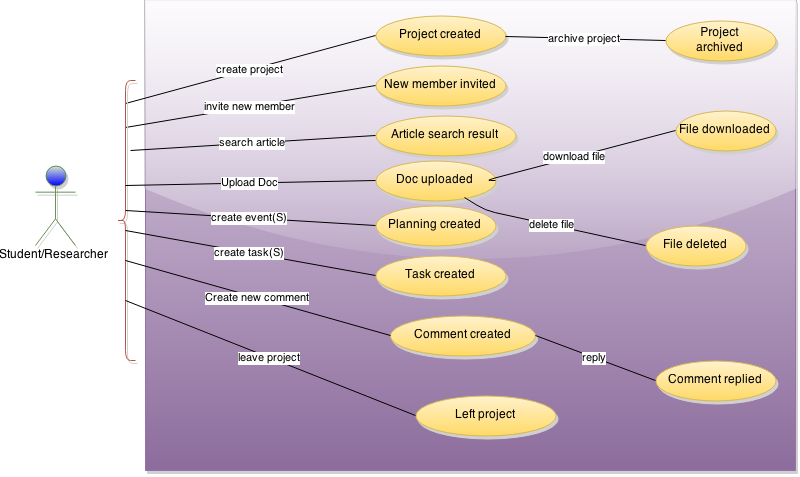
\includegraphics[scale=0.3]{./img/dsgn_img/USECASE1.png}	
\end{center}

% subsection subsection_name (end)

\subsubsection{Reviewer User} 
\begin{center}
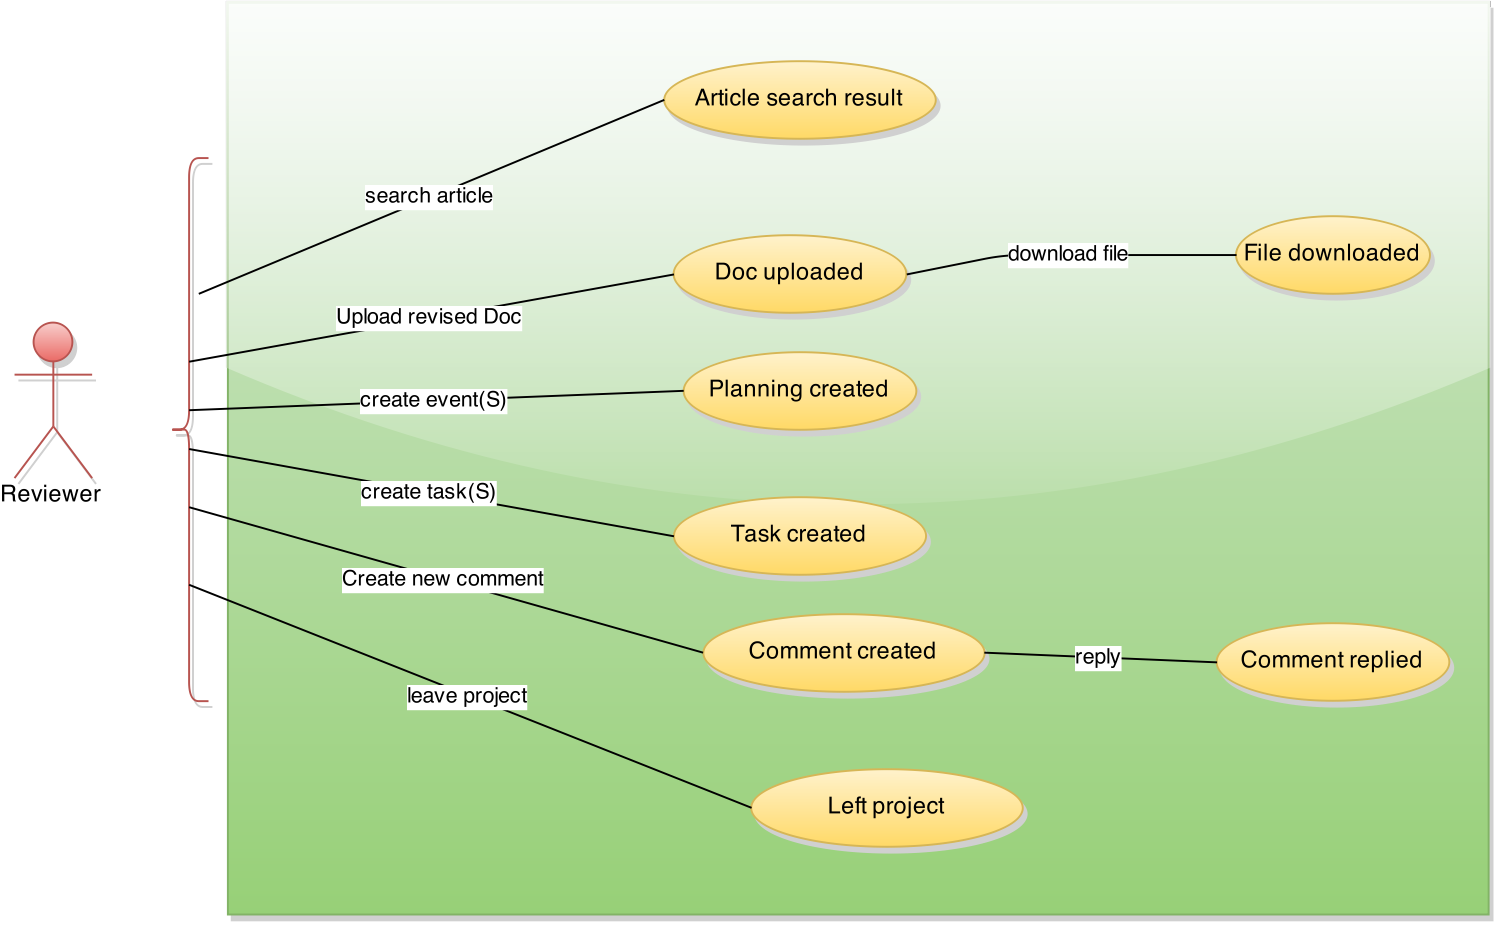
\includegraphics[scale=0.3]{./img/dsgn_img/USECASE2.png}
	
\end{center}

\subsubsection{Administrator User} 
\begin{center}
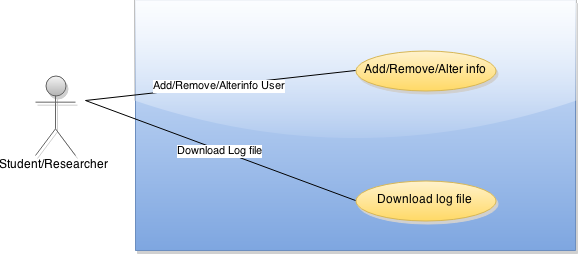
\includegraphics[scale=0.3]{./img/dsgn_img/USECASE3.png}
	
\end{center}
% subsection list_of_use_cases (end)

% subsection actors (end)

\section{System Architecture} % (fold)
\label{sec:system_architecture}
 In this section, MVC design of the system is shown and will be discussed. MVC is chosen to be very suitable for web architecture since it promises low coupling and high cohesion between components of the systems and gives room for easier extension or modification of a specific component without bothering the rest.
\subsection{Architectural Design} % (fold)
\label{sub:arichtectural_design}
% Develop a modular program structure and explain the relationships between the modules to achieve  the  complete  functionality of the  system. This is a  high level overview  of how responsibilities of the system were partitioned and then assigned to subsystems. Identify each 
% high level subsystem and  the  roles or responsibilities assigned to it. Describe  how  these subsystems col aborate with each other in order to achieve the desired functionality. Don’t go 
% into too much detail about the individual subsystems. The main purpose is to gain a general understanding  of how  and why the system was decomposed, and  how the  individual parts work together. Provide a diagram showing the major subsystems and data repositories and their interconnections. Describe the diagram if required

In the app folder of this application, there are three packages defined. namely models, view and controller. 
\begin{center}
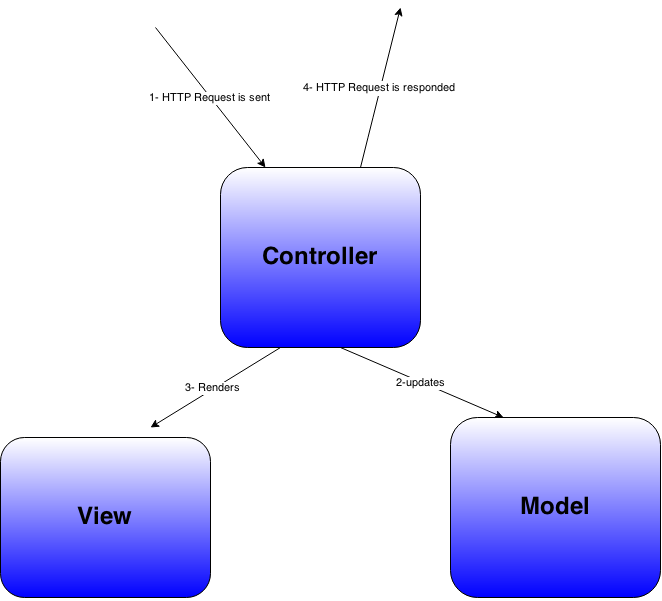
\includegraphics[scale=0.3]{./img/dsgn_img/MVCdiag.png}
	
\end{center}

Image above is showing that these the system architecture divides into three separate layers. The model which is representation of information, THe view that makes these information available for the user to interact and Controller which responds to user actions and processes them. In the next section we will explain more in-dept about each layer and it's sub-components.

\subsection{Model} % (fold)
\label{sub:design_rationale}

\subsubsection{RElational Model Diagram}
\begin{center}
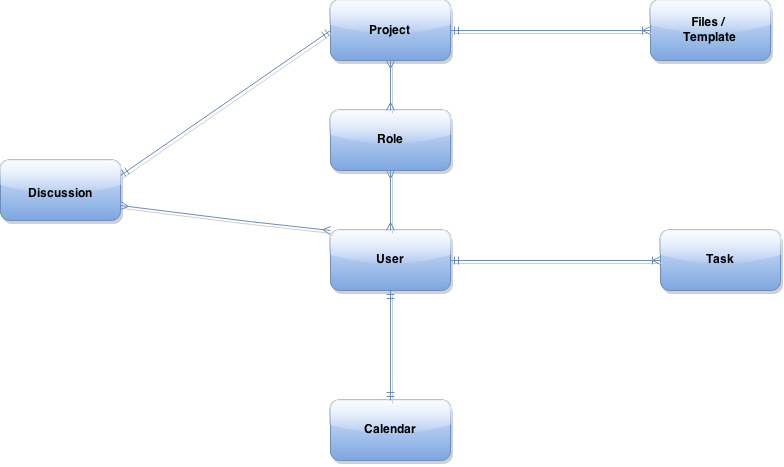
\includegraphics[scale=0.3]{./img/dsgn_img/RMA.png}
	
\end{center}

\subsubsection{Model description}

\subsection{View} % (fold)

\subsubsection{Screen Images} % (fold)

\subsubsection{Screen Objects and Actions} % (fold)



\subsection{Controller} % (fold)

